%\documentclass{article}
%\usepackage{graphicx,subfigure}
%\begin{document}

\begin{figure}[!h]
  \centering
  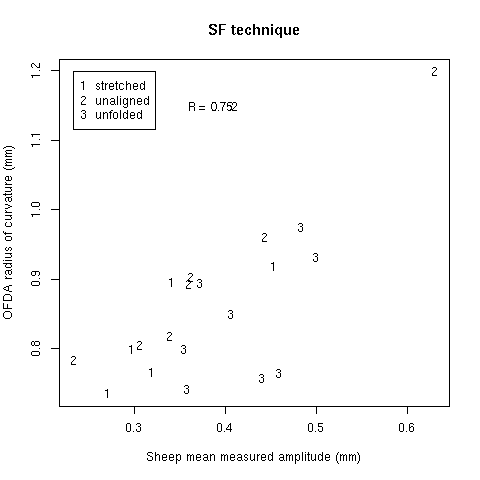
\includegraphics[width=1.0\textwidth]{figofdaradsfampl.png}
%   ofdaradsfampl.png is original 
  \caption{Correlation between sheep means for Amplitude measured by the SF technique and radius of curvature measured by OFDA staple scanning technique. CrimpType identified for each sheep. Means are averages over 30 waves per fibre.}
  \label{fig:ofdaradsfampl}
\end{figure}

%\end{document}

